\documentclass[twoside,10pt]{report}
\newcommand{\docTitle}{Hw 13}
\usepackage{/Users/bradenhoagland/latex/math2}

%\renewcommand{\theenumi}{\alph{enumi}}

\begin{document}
%\tableofcontents

\begin{exer}[]
	What happens if you join two M{\"o}bius strips together along their circle boundaries? Show this in two ways:
\begin{enumerate}
	\item By using Theorem 4.10.
	\item By cutting and gluing squares with arrows on their edges.
\end{enumerate}
\end{exer}

\begin{enumerate}
	\item Since the Klein bottle $K$ can be represented by
		\begin{figure}[H]
			\centering
			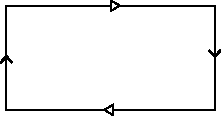
\includegraphics[scale=1]{fig/k.pdf}
		\end{figure}
		we can calculate its Euler characteristic as $\chi(K)=0$ (1 vertex, 2 edges, 1 face).

		Note that in order for a M\"obius strip to be a manifold, it cannot have a boundary. Thus by ``M\"obius strip" we mean the following diagram with open boundary.
		\begin{figure}[H]
			\centering
			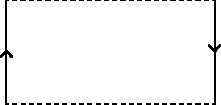
\includegraphics[scale=1]{fig/m-open.pdf}
		\end{figure}
Once we glue two strips together, though, this open bit goes away and we're left with a compact surface.

Using this image, we can calculate that the Euler characteristic of a M\"obius strip is 0 (2 vertices, 3 edges, 1 face). Denote the glued-together M\"obius strips by $M$, then the rectangular decomposition of $M$ into M\"obius strips shows that $\chi(M)=0$.

		Both $K$ and $M$ are connected, compact, and non-orientable. Then since both have Euler characteristic 0, they are diffeomorphic by Theorem 4.10. Thus the Klein bottle is just two M\"obius strips glued together along their boundaries.

	\item Given a M\"obius strip
		\begin{figure}[H]
			\centering
			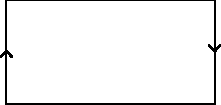
\includegraphics[scale=1]{fig/m.pdf}
		\end{figure}
		it's not visually clear how to glue another M\"obius strip to this. But we can cut the strip as follows.
		\begin{figure}[H]
			\centering
			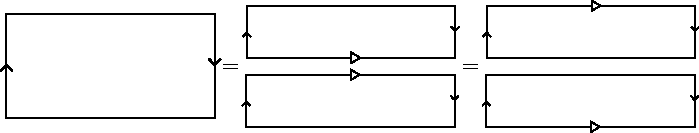
\includegraphics[scale=1]{fig/m-split.pdf}
		\end{figure}
		Then it's clear how to glue this to another (whole) M\"obius strip.
		\begin{figure}[H]
			\centering
			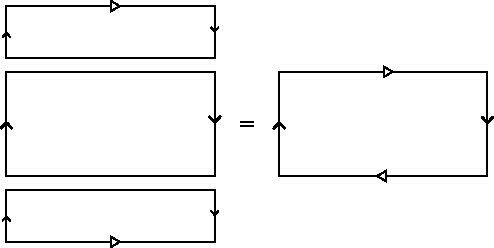
\includegraphics[scale=1]{fig/2m.pdf}
		\end{figure}
		This is exactly a Klein bottle.
		
\end{enumerate}

\end{document}
